\documentclass{standalone}
\usepackage{tikz}
\usetikzlibrary{positioning, decorations.pathreplacing}

\begin{document}
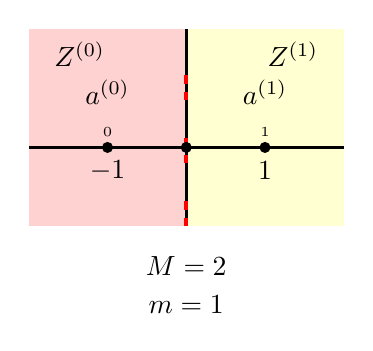
\begin{tikzpicture}

% Define colors
\definecolor{myred}{RGB}{255, 210, 210}
\definecolor{myyellow}{RGB}{255, 255, 210}

% Draw the rectangles
\fill[myred] (-2, 0) rectangle (0, 2.5);
\fill[myyellow] (0, 0) rectangle (2, 2.5);

% Vertical line in the middle
\draw[very thick] (0, 0) -- (0, 2.5);
% Draw the dashed lines in red
\draw[red, ultra thick, dashed] (0, 0) -- (0, 0.4);
\draw[red, ultra thick, dashed] (0, 0.8) -- (0, 1.2);
\draw[red, ultra thick, dashed] (0, 1.6) -- (0, 2);

% Draw the horizontal line
\draw[thick] (-2, 1) -- (2, 1);

% Draw the nodes
\fill (0, 1) circle (2pt);
\fill (-1, 1) circle (2pt);
\fill (1, 1) circle (2pt);

% Add labels
\node at (-1, 1.2) {\textnormal{\tiny $0$}};
\node at (1, 1.2) {\textnormal{\tiny $1$}};

\node at (-1, 0.7) {$-1$};
\node at (1, 0.7) {$1$};

\node at (-1, 1.7) {$a^{(0)}$};
\node at (1, 1.7) {$a^{(1)}$};

\node[above right] at (-1.8, 1.9) {$Z^{(0)}$};
\node[above left] at (1.8, 1.9) {$Z^{(1)}$};

% Add the bottom text
\node at (0, -0.5) {$M=2$};
\node at (0, -1) {$m=1$};

\end{tikzpicture}
\end{document}


